\section{Experimental Validation}
\label{sec:exp}

The experiments evaluate RoCBF-SF as a real-time safety layer in an industrial DCS control loop. The validation addresses four issues: GP residual correction under model mismatch, robustness-factor calibration, sampling-budget fit, and post-retrofit execution evidence from plant historian and controller-log records.

\subsection{Boiler-Turbine Benchmark and Filter Comparisons}

The benchmark is a fifth-order nonlinear model of the boiler-turbine coordinated control loop of an ultra-supercritical power unit with state $x = [r_B, p_m, h_m, N_e, \tau_f]^\top$ and three control inputs. The enforced limits are pressure ($m=2$, 13--24\,MPa), separator enthalpy ($m=1$, 2670--2830\,kJ/kg), and generator active-power tracking around the dispatch target ($m=1$, $N_{\mathrm{ref}}\pm50$\,MW). Table~\ref{tab:safety} tests the $\Delta g=0$ structural scope of Theorem~\ref{thm:1}: the rollout plant and the filter use the same fixed input matrix, so mismatch enters through drift residuals. The finite rollouts do not by themselves verify the theorem's uniform residual and derivative-bound assumptions.

Six perturbation scenarios model heat-absorption loss (S1), feedwater-induced pressure disturbance (S2), coupled state-dependent drift (S3), nonlinear fouling (S4), valve-related process drift (S5), and fuel-quality variation (S6). S5 is represented as equivalent state drift rather than as an input-gain fault, so the $\Delta g=0$ condition is maintained. S5 and S6 also perturb the extended power/fuel-delay dynamics of the fifth-order model.

To isolate the safety layer in the $\Delta g=0$ validation, the fixed-proposal and HOCBF rows in Table~\ref{tab:safety} use the same seeded, bounded upstream deviation command and differ only in the downstream filter. Each method-condition cell contains five independent 500-sample rollouts (2500 controller samples). All GP variants use 500 scenario-specific training transitions, the common input/output vector $[p_m,h_m,N_e]^\top$, and a frozen training-input z-score transform. The QP is solved with qpax 0.1.3 in 64-bit arithmetic using row scaling, box constraints, and an acceptance requirement of solver convergence, finite primal values, and maximum normalized primal residual no greater than $10^{-6}$. Rejected QP candidates revert to the live upstream proposal and are counted as fallback events. A raw-margin numerical tolerance of $10^{-2}$ is used only for counting binary state-limit violations; unrounded minimum margins remain in the result files.

NMPC is evaluated under the same $\Delta g=0$ rollout conditions as an optimization-based reference. It solves a warm-started SLSQP problem with horizon $N{=}5$, deviation-input bounds $v_i\in[-10,10]$, the same six process constraints, a stabilized linear prediction model, and additive disturbance correction. The output and input weights are $\mathrm{diag}(1.0,0.001,0.01)$ and $\mathrm{diag}(0.01,0.01,0.01)$, respectively; the disturbance-estimator gain is 0.5, and SLSQP uses \texttt{maxiter}$=50$ and \texttt{ftol}$=10^{-4}$. Every one of the 17{,}500 NMPC solves in Table~\ref{tab:safety} converged and passed a $10^{-6}$ prediction-constraint residual check.

The safety tables use a sample-level violation rate at the controller instants,
\begin{equation}
R_{\mathrm{viol}}(\eta) =
\frac{\sum_{s=1}^{N_{\mathrm{seed}}}\sum_{e=1}^{N_{\mathrm{ep}}}\sum_{t=1}^{N_{\mathrm{step}}}
\mathbf{1}\{\min_j h_j(x_{s,e,t}) < -\eta\}}
{N_{\mathrm{seed}}N_{\mathrm{ep}}N_{\mathrm{step}}},
\label{eq:sample_violation_rate}
\end{equation}
where a sample is counted once if any enforced pressure, separator-enthalpy, or power barrier is below the stated numerical tolerance $\eta$ at that controller sampling instant. Table~\ref{tab:safety} uses $\eta=10^{-2}$ in raw barrier units to avoid counting QP boundary-roundoff as physical violation; the later stress-test diagnostics use the tolerance stated in their result files or captions. This is not an episode-level probability. A single-rollout diagnostic such as 4/300 in Fig.~\ref{fig:process_response} is reported only for that diagnostic rollout. Table~\ref{tab:safety} aggregates controller samples across seeds and rollouts for the $\Delta g=0$ validation.

\subsection{Closed-Loop Safety and Process Response}

\begin{table}[htbp]
    \centering
    \caption{Primary $\Delta g=0$ validation: sample-level constraint violation rate (\%) at controller instants under a fixed upstream deviation proposal, computed by Eq.~\eqref{eq:sample_violation_rate} with a raw-margin numerical tolerance of $10^{-2}$. Each cell aggregates five 500-sample rollouts, i.e., 2500 controller samples. The full implemented-margin row tests the conservative $\epsilon_\kappa=1.0$ endpoint under actuator limits; it is not the recommended commissioned operating point.}
    \label{tab:safety}
    \small
    \resizebox{0.98\textwidth}{!}{%
    \begin{tabular}{>{\raggedright\arraybackslash}p{0.30\textwidth}*{7}{>{\centering\arraybackslash}p{0.075\textwidth}}}
        \toprule
        Method & Nom. & S1 & S2 & S3 & S4 & S5 & S6 \\
        \midrule
        Unfiltered fixed upstream proposal & 4.48 & 78.64 & 68.56 & 67.28 & 68.56 & 68.56 & 78.64 \\
        HOCBF, no GP ($m{=}2,1,1$) & 0.00 & 78.64 & 68.56 & 67.28 & 68.56 & 68.56 & 78.64 \\
        NMPC ($N{=}5$) & 0.00 & 0.20 & 0.20 & 0.40 & 0.20 & 0.20 & 0.20 \\
        GP-HOCBF mean-only ($\epsilon_\kappa{=}0$) & 0.00 & 0.00 & 0.00 & 1.44 & 0.00 & 0.00 & 0.00 \\
        RoCBF-SF commissioned ($\epsilon_\kappa{=}0.02$ in S3; 0 otherwise) & 0.00 & 0.00 & 0.00 & 0.00 & 0.00 & 0.00 & 0.00 \\
        Full implemented-margin endpoint ($\epsilon_\kappa{=}1.0$) & 0.00 & 0.00 & 0.00 & 16.76 & 0.48 & 0.00 & 0.00 \\
        \bottomrule
    \end{tabular}
    }
\end{table}

Table~\ref{tab:safety} reports the drift-only $\Delta g=0$ validation. The unfiltered proposal violates 10{,}756 of 15{,}000 perturbation samples. Correct relative degree removes all 112 nominal violations but does not compensate drift mismatch: no-GP HOCBF retains the same 10{,}756 perturbation-sample violations. GP mean correction reduces this count to 36/15{,}000, all in S3. The scenario-wise commissioned row applies the independently selected $\epsilon_\kappa=0.02$ in S3 and 0 otherwise, giving 0/17{,}500 observed violations across the nominal and six mismatch conditions. Each condition is a separate offline commissioning regime with its own frozen scenario-specific GP; this row compares commissioned operating points across prescribed residual regimes rather than switching $\epsilon_\kappa$ by observing the true scenario online. NMPC is also effective, with 35/17{,}500 violations and no solver failure, but does not eliminate the short boundary transients in the six mismatch cases.

The full implemented-margin row shows why $\epsilon_\kappa$ must be commissioned rather than set mechanically to its largest value. The endpoint remains safe in nominal, S1, S2, S5, and S6, but it produces 419 S3 violations and 12 S4 violations when the actuator-bounded robust QP loses feasibility. This does not contradict Theorem~\ref{thm:1}, which requires both full-row feasibility and independently valid residual and derivative bounds.

Table~\ref{tab:qp_endpoint_diagnostic} makes that feasibility mechanism explicit for S3. The revised experiment records every QP attempt, rejected candidate, fallback, intervention, and normalized residual. The commissioned row has four rejected initial-step QPs but no ensuing state-limit violation; the full implemented-margin endpoint rejects 628 of 2500 QPs and reverts to the upstream command in those cycles.

\begin{table}[htbp]
    \centering
    \caption{S3 solver and intervention diagnostics for the primary $\Delta g=0$ validation. Each row contains 2500 controller samples. QP rejection requires non-convergence, a non-finite candidate, or normalized primal residual above $10^{-6}$; the live upstream proposal is used on a rejected cycle. NMPC uses its own horizon optimization and is therefore omitted from the projection-intervention comparison.}
    \label{tab:qp_endpoint_diagnostic}
    \small
    \resizebox{\textwidth}{!}{%
    \begin{tabular}{>{\raggedright\arraybackslash}p{0.29\textwidth}*{4}{>{\centering\arraybackslash}p{0.16\textwidth}}}
        \toprule
        S3 method & Violation & QP rejected & Fallback & QP intervention \\
        \midrule
        HOCBF, no GP & 1682/2500 (67.28\%) & 0/2500 & 0/2500 & 4.48\% \\
        GP-HOCBF mean-only & 36/2500 (1.44\%) & 0/2500 & 0/2500 & 67.08\% \\
        RoCBF-SF, $\epsilon_\kappa=0.02$ & 0/2500 & 4/2500 & 4/2500 & 67.12\% \\
        Full implemented-margin endpoint & 419/2500 (16.76\%) & 628/2500 & 628/2500 & 51.12\% \\
        \bottomrule
    \end{tabular}
    }
\end{table}

The results indicate a mechanism hierarchy: correct HOCBF structure handles nominal constraint geometry, GP residual correction is the principal mismatch-compensation mechanism, and $\epsilon_\kappa$ is a finite-sample feasibility--safety trade-off. The following diagnostics separate the time-domain mechanism, residual-model evidence, data-quality gate, and tune/test calibration result.

\begin{figure}[htbp]
    \centering
    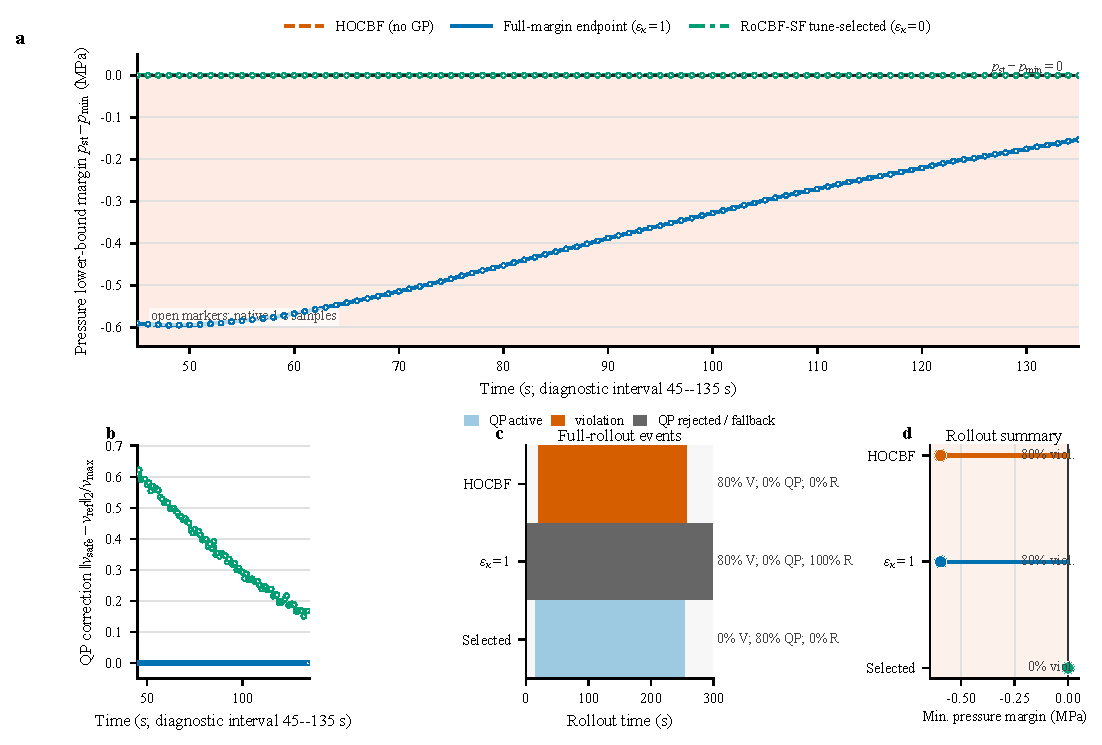
\includegraphics[width=0.95\textwidth]{figures/Figure_6_process_response.pdf}
    \caption{Closed-loop mechanism for representative seed~3 under the drift-only S3 perturbation. \textbf{(a,b)} Enthalpy safety margin and normalized QP correction over the 45--135\,s interval containing the onset and largest excursion. The shaded region marks violation of the lower enthalpy constraint. \textbf{(c)} Full 300\,s event record. \textbf{(d)} Full-rollout minimum enthalpy margin and sample-level violation rate; the symmetric-log horizontal scale resolves the two near-zero margins while retaining the large no-GP excursion. Lines in (a,b) are interpolated on a 0.1\,s display grid only for visual continuity; open markers are the native 1\,s controller samples, and all statistics use native samples and the $10^{-2}$ counting tolerance defined in Eq.~\eqref{eq:sample_violation_rate}.}
    \label{fig:process_response}
\end{figure}

In this representative rollout, the no-GP HOCBF records 203/300 violations, GP mean correction reduces the count to 30/300, and the calibrated setting records 0/300. The corresponding minimum enthalpy margins are $-51.993$, $-0.01996$, and $+0.01028$\,kJ/kg. This single-trajectory diagnostic illustrates the mechanism and is not used in place of the five-seed aggregate in Tables~\ref{tab:safety} and \ref{tab:qp_endpoint_diagnostic}.

Figure~\ref{fig:process_response} shows the enthalpy bottleneck directly in a representative S3 rollout. HOCBF without GP correction produces 203/300 violating samples and a minimum enthalpy margin of $-51.993$\,kJ/kg. GP mean correction limits the excursion to $-0.01996$\,kJ/kg but still leaves 30 samples below the stated numerical tolerance, whereas the calibrated $\epsilon_\kappa=0.02$ margin keeps the minimum positive at $+0.01028$\,kJ/kg. The correction and event panels show that this change is produced by sustained QP intervention rather than by a different upstream proposal.

\begin{figure}[htbp]
    \centering
    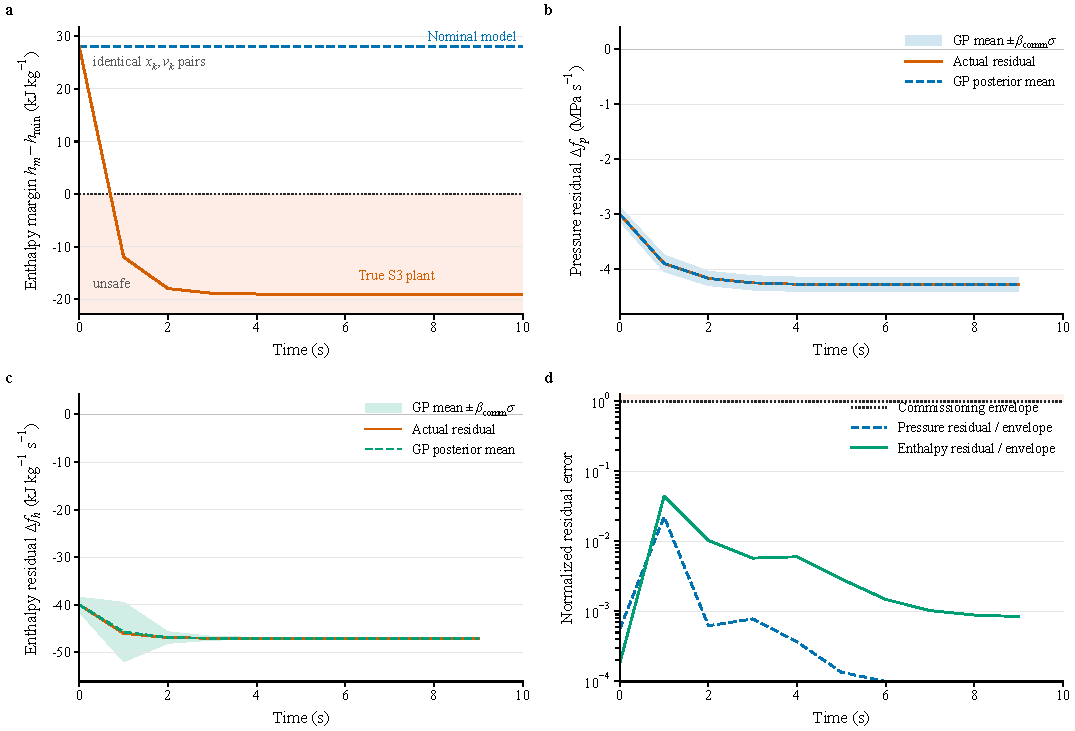
\includegraphics[width=0.95\textwidth]{figures/Figure_8_model_mismatch.pdf}
    \caption{Direct model-mismatch diagnosis under the drift-only S3 perturbation. \textbf{(a)} Nominal and true one-step enthalpy-margin responses from identical state-input pairs. \textbf{(b,c)} Pressure and enthalpy residual rates compared with the scenario-specific GP posterior mean and commissioning envelope ($\mu_{\mathrm{GP}}\pm\beta_{\mathrm{comm}}\sigma_{\mathrm{GP}}$, $\beta_{\mathrm{comm}}=12.967$, $N=500$). \textbf{(d)} Posterior residual error normalized by that implemented envelope; values below one lie inside the plotted envelope, not a separately established uniform GP confidence set.}
    \label{fig:model_mismatch}
\end{figure}

Figure~\ref{fig:model_mismatch} makes the model mismatch explicit. For the same state and zero-deviation input, the nominal model predicts a next-step enthalpy margin of 28.0\,kJ/kg, whereas the S3 plant drops to $-12.0$\,kJ/kg. The pressure and enthalpy panels show that this discrepancy is structured and learnable: the GP posterior mean tracks the realized drift residual, and the remaining error stays inside the implemented commissioning envelope in this diagnostic. The filter therefore corrects a measured residual structure before applying the commissioned margin.

\begin{figure}[htbp]
    \centering
    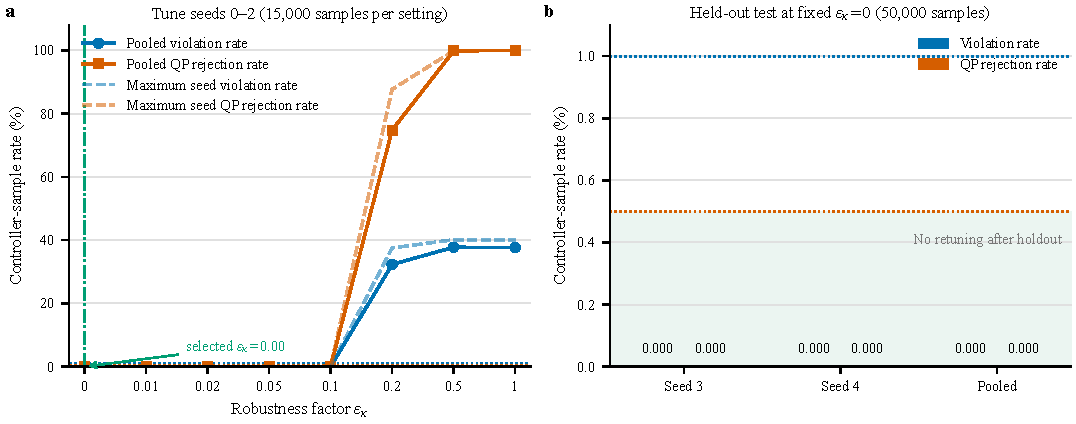
\includegraphics[width=0.95\textwidth]{figures/Figure_2.pdf}
    \caption{Tune/test calibration of $\epsilon_\kappa$ under S3. \textbf{(a)} Pooled and maximum-per-seed violation and QP-rejection rates for tune seeds 0--2 (15{,}000 native controller samples per setting). The predeclared rule selects the smallest value with pooled and per-seed violation below 1\% and QP rejection below 0.5\%. \textbf{(b)} Results for held-out seeds 3--4 after fixing $\epsilon_\kappa=0.02$; no retuning used the 50{,}000 holdout samples.}
    \label{fig:traj}
\end{figure}

Figure~\ref{fig:traj} separates calibration from confirmation. On tune seeds 0--2, $\epsilon_\kappa=0$ gives 412/15{,}000 violations (2.747\%). The smallest setting passing both gates is 0.02, with 19/15{,}000 violations (0.127\%) and 20/15{,}000 rejected QPs (0.133\%). After fixing this value, held-out seeds 3--4 give 66/50{,}000 violations (0.132\%) and 72/50{,}000 rejected QPs (0.144\%), with both individual seeds below the same gates. The Wilson values in the Supplemental Material are descriptive Bernoulli-reference bounds because adjacent controller samples are serially correlated. These results define a finite-sample operating point, not a zero-violation guarantee.

\subsection{Robustness-Factor Commissioning}
\label{sec:kappa}

\begin{figure}[htbp]
    \centering
    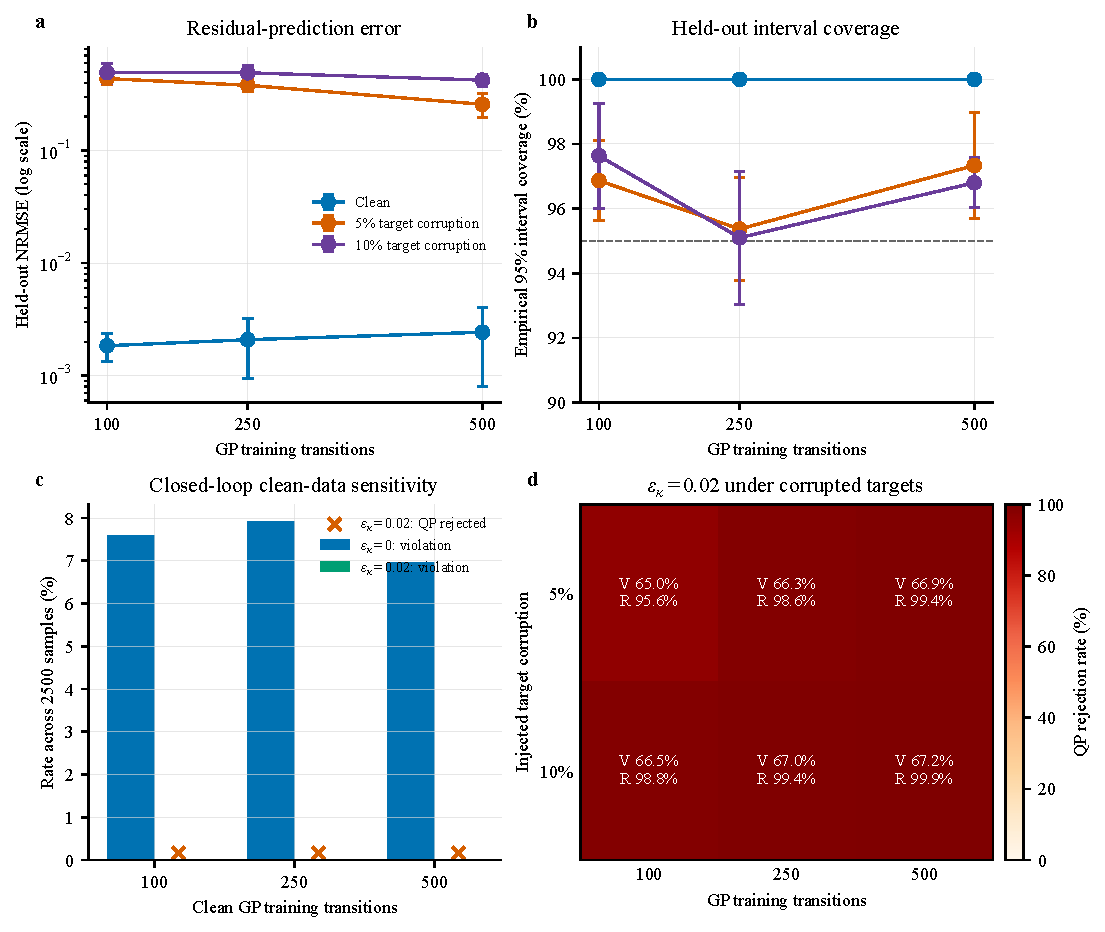
\includegraphics[width=0.95\textwidth]{figures/Figure_GP_data_sensitivity.pdf}
    \caption{Controlled GP training-data sensitivity under S3. \textbf{(a,b)} Held-out residual NRMSE and empirical 95\% interval coverage for 100, 250, and 500 selected transitions. Target corruption replaces a fixed training fraction with signed three-standard-deviation offsets. \textbf{(c,d)} Closed-loop violation and QP-rejection diagnostics under clean and corrupted training data. Each point aggregates five 500-sample rollouts. The 5\% and 10\% levels are synthetic fault-injection tests, not estimates of plant-data quality.}
    \label{fig:gp_data_sensitivity}
\end{figure}

Figure~\ref{fig:gp_data_sensitivity} tests the GP commissioning gate rather than treating every fitted model as deployable. Across 100, 250, and 500 clean training transitions, held-out NRMSE remains between 0.00184 and 0.00243, interval coverage is 100\%, and $\epsilon_\kappa=0.02$ gives 0/2500 violations with 0.16\% QP rejection at each size. Controlled label corruption raises NRMSE by approximately two orders of magnitude and drives QP rejection to 95.64--99.88\%; fallback to the upstream proposal then produces 64.96--67.20\% violation. These deliberately corrupted models fail the pre-enable quality and feasibility gate. The complete aggregation is reported in the Supplemental Material.

\subsection{Real-Time Computation}
\label{sec:comp}

The deployment configuration specifies an AMD EPYC Embedded 4565P processor, 64\,GB (2$\times$32\,GB) DDR5-5600 ECC memory, openEuler 24.03 LTS, Python 3.11, qpax 0.1.3 for the online QP, SciPy 1.17.1, Kubernetes workload management, and Modbus TCP data exchange with the DCS. The online controller executes every 1\,s. The production-validation files are controller exports at 5\,s spacing; therefore, counts reported from those files refer to exported records rather than every internal controller cycle.

The implemented benchmark filter and NMPC reference both fit within the 1\,s budget; scenario-level timing and GP storage/training complexity are reported in the Supplemental Material. Field execution time is the deployment-relevant measurement and is reported with the confirmed controller exports in Section~\ref{sec:historian}.

\subsection{Measured Plant Evidence: Envelope, Matched Windows, and Controller Logs}
\label{sec:historian}

The simulation benchmark establishes the closed-loop mechanism: GP residual correction closes most of the model mismatch, $\epsilon_\kappa$ must be calibrated by uncertainty structure, and the compiled filter satisfies the 1\,s sampling budget. Plant data then connect the same design to measured operation. Historian records define the operating envelope, load-matched windows compare pre- and post-retrofit response, and confirmed original plant-controller exports document both routine full-QP execution and a bounded reduced-QP recovery mode under measured operating conditions.

Figure~\ref{fig:production_historian} uses a bounded historian snapshot from the 660\,MW unit as an operating-envelope check. The grey envelope uses an approximately 24\,h loaded operating window from 1~July~2026 02:33 to 2~July~2026 02:28 local time ($n=288$ at 300\,s spacing). The colored overlays place three post-retrofit low-to-mid-load historian windows within that measured load--pressure range. This record documents measurement availability and operating variability; the original 5\,s historian records in Fig.~\ref{fig:retrofit_historian} provide the dynamic resolution for retrofit comparison.

\begin{figure}[htbp]
    \centering
    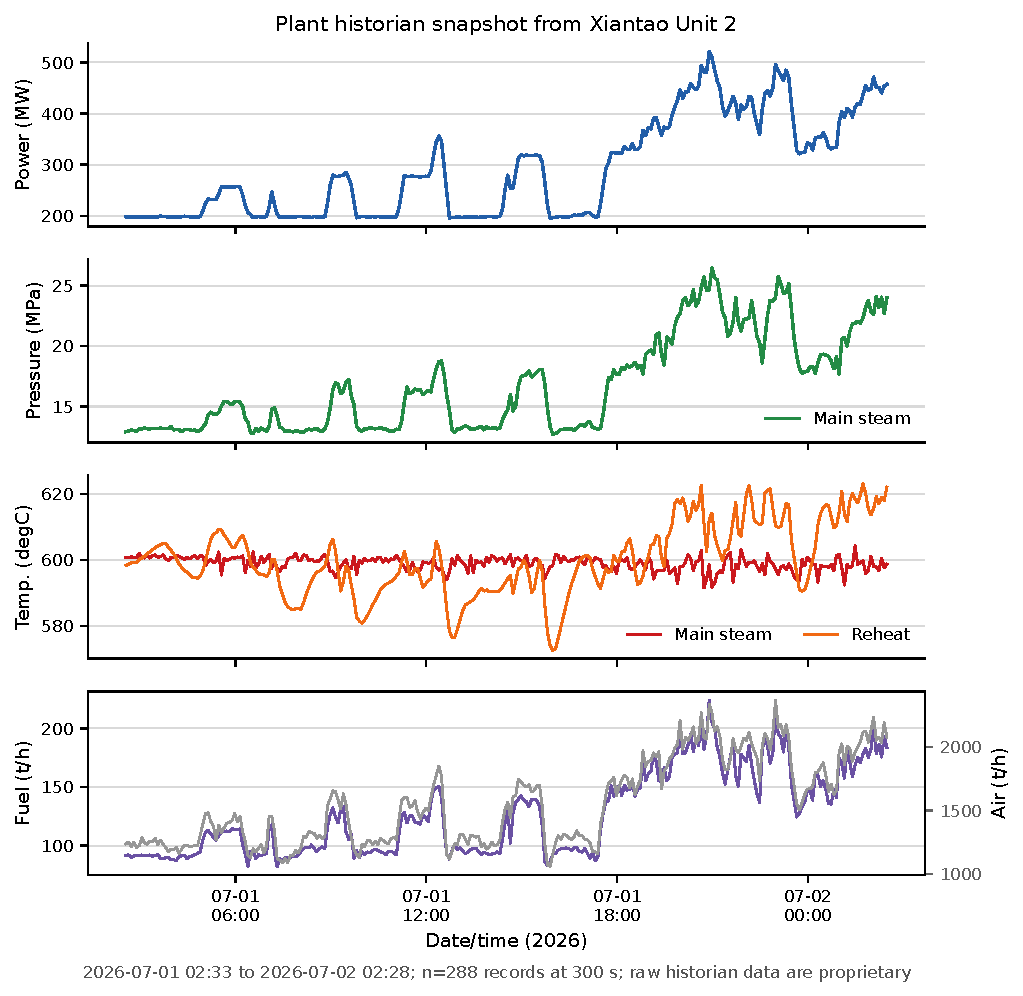
\includegraphics[width=0.95\textwidth]{figures/Figure_9_production_historian.pdf}
    \caption{Plant-historian operating-envelope check from the 660\,MW ultra-supercritical unit. \textbf{(a)} Five-minute historian samples define the measured load--pressure envelope over an approximately 24\,h loaded interval; colored boxes and markers locate three two-hour post-retrofit low-to-mid-load historian windows. \textbf{(b,c)} The same windows are shown as load and pressure ranges against the 24\,h min--max and p05--p95 envelopes. The figure places these historian windows within measured plant operation.}
    \label{fig:production_historian}
\end{figure}

During this interval, generator active power varied from 195.7 to 520.8\,MW and main-steam pressure ranged from 12.70 to 26.47\,MPa. This 24\,h range is a historian operating-envelope measurement, not the safety-filter constraint envelope. The three colored overlays in Fig.~\ref{fig:production_historian} are low-to-mid-load historian context windows (MW01--MW03), whose main-steam-pressure ranges are 13.21--19.15\,MPa. They do not supply controller-internal QP fields. Load was strongly correlated with pressure ($r=0.986$) and fuel flow ($r=0.980$), confirming pressure--combustion coupling during load following. The MW04--MW06 controller exports analyzed below provide the separate execution evidence at 480.7--629.7\,MW (72.8--95.4\% of nameplate power).

The unit chronology permits a load-matched commissioning comparison. The 660\,MW unit used traditional PID before 21~May~2026, was shut down from 21~May to 24~June~2026, and restarted with the proposed RoCBF-SF-based strategy after 24~June~2026. The outage included extensive routine plant maintenance in addition to integration of the proposed algorithm. We screened historical pre-retrofit windows from 2024--2025 and post-retrofit windows after the first 24\,h of restart, retaining loaded operation and matching by load trajectory. The audit retained 1950 two-hour windows during loaded operation. Across this matched-window cohort, the period-median pressure setpoint-residual standard deviation and 95th-percentile absolute residual decrease by 12.6\% and 23.4\%, respectively. The representative pair below uses the original 5\,s historian samples, with historian files, source timestamps, and metric JSON preserved in the evidence package. Because routine maintenance occurred during the same outage, the plant-response comparison is interpreted as observational evidence associated with the documented retrofit under matched load movement, rather than as a standalone estimate of the algorithm's causal effect. Confirmed original plant-controller exports provide the separate evidence that RoCBF-SF executed after restart.

\begin{figure}[htbp]
    \centering
    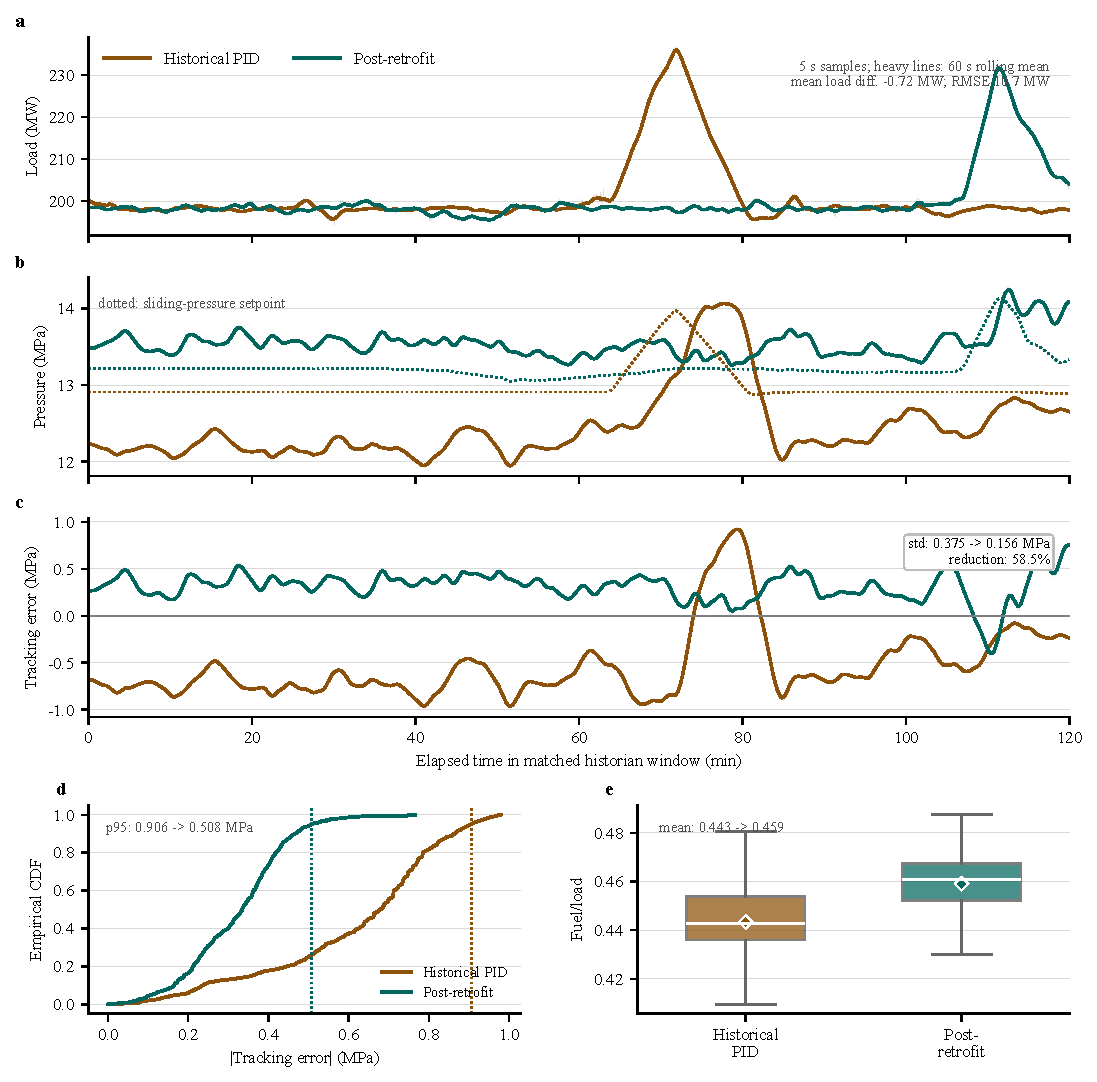
\includegraphics[width=0.95\textwidth]{figures/Figure_10_production_retrofit_evidence.pdf}
    \caption{Matched plant-historian retrofit-window diagnostic from the 660\,MW ultra-supercritical unit. The historical PID window is 5~November~2025 11:00--12:59:55 local time; the post-retrofit window is 25~June~2026 12:30--14:29:55 local time. Both windows contain 1440 original 5\,s historian samples. \textbf{(a)} Generator active-power trajectories used for matching; the mean-load difference is $-0.72$\,MW and the load-profile RMSE is 10.7\,MW. \textbf{(b)} Main-steam pressure and the sliding-pressure setpoint. \textbf{(c)} Pressure tracking error, $p_{\mathrm{main}}-p_{\mathrm{set}}$; the sample-level standard deviation decreases from 0.375 to 0.156\,MPa. \textbf{(d)} Empirical CDF of absolute pressure tracking error; dotted lines mark the 95th percentile, which decreases from 0.906 to 0.508\,MPa. \textbf{(e)} Fuel/load distribution for the combustion-side operating context; boxes show median, IQR, and 1.5$\times$IQR whiskers, and diamonds show means. Light traces are original samples and heavy traces are 60\,s rolling means for readability; all reported metrics use the original 5\,s samples.}
    \label{fig:retrofit_historian}
\end{figure}

Figure~\ref{fig:retrofit_historian} reports a high-resolution matched pair. The two-hour windows have mean load within 1\,MW and load-profile RMSE of 10.7\,MW. Pressure tracking-error standard deviation decreases by 58.5\% after retrofit, from 0.375 to 0.156\,MPa, and the 95th-percentile absolute error decreases from 0.906 to 0.508\,MPa. The fuel/load proxy is higher after retrofit (0.443 to 0.459), so the comparison was not obtained under lower combustion-side demand. The load-matched result documents improved pressure response after the retrofit under comparable load movement. Because routine outage maintenance occurred concurrently, this comparison does not by itself attribute the entire improvement to RoCBF-SF; the controller exports independently verify online execution of the proposed filter. The plant evidence complements the controlled model-mismatch tests in Figs.~\ref{fig:process_response}--\ref{fig:model_mismatch}.

The same 5\,s historian query includes main/reheat temperature, air--coal ratio channels, mode/fallback indicators, and turbine-valve demand. Main-steam temperature variability decreases from 2.245 to 0.915\textdegree{}C, while reheat-temperature variability and air--coal ratio dispersion increase, showing that the post-retrofit interval is not uniformly easier. These historian diagnostics are then paired with the post-retrofit controller-log export in Fig.~\ref{fig:controller_log_validation}; the historical PID window is not assigned QP/CBF fields because no online safety filter was running before retrofit.

\begin{figure}[htbp]
    \centering
    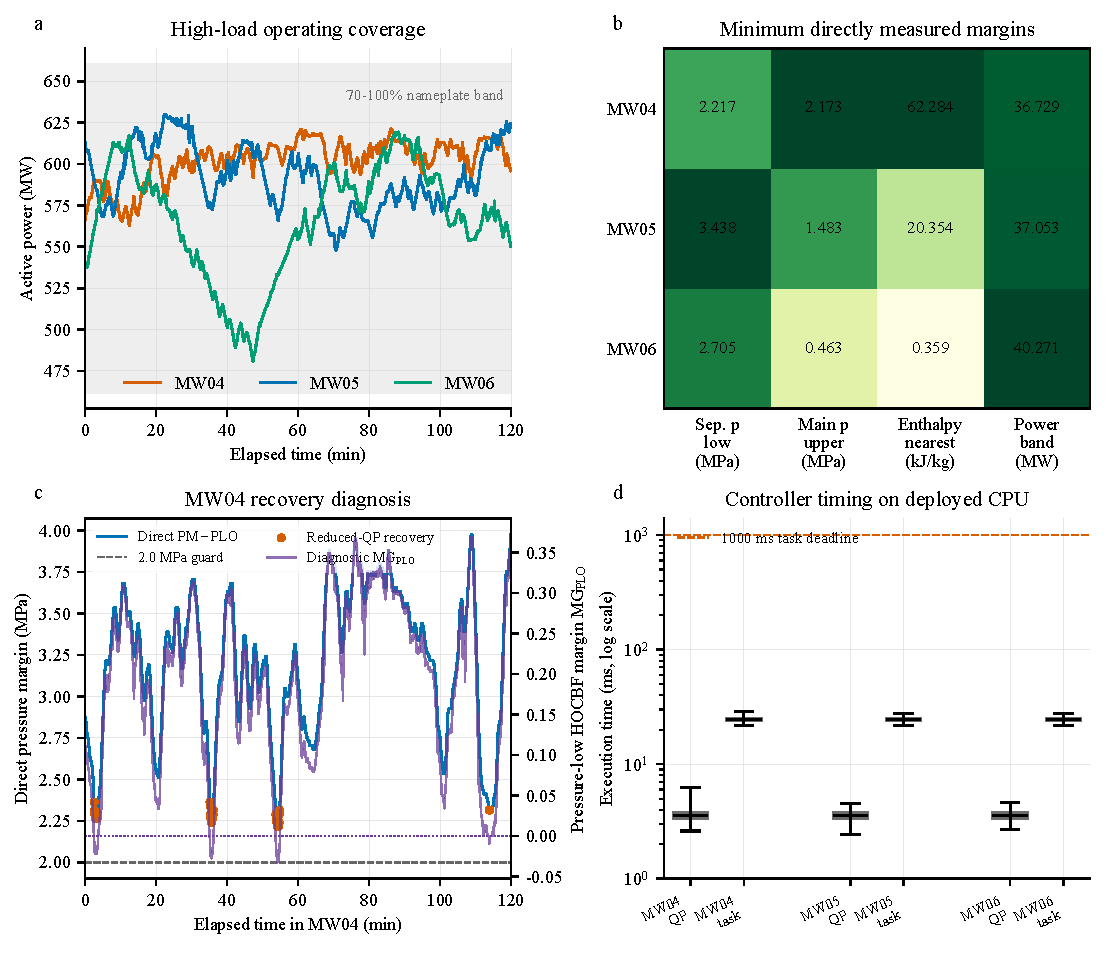
\includegraphics[width=0.95\textwidth]{figures/Figure_11_controller_log_validation.pdf}
    \caption{High-load plant-controller evidence from three post-retrofit two-hour windows, each containing 1440 records exported at 5\,s spacing from a controller executing at 1\,s. \textbf{(a)} Generator active power; the shaded band denotes 70--100\% of the 660\,MW nameplate rating. \textbf{(b)} Minimum directly measured margins to the separator-pressure lower bound, main-steam-pressure upper replay bound, nearest separator-enthalpy bound, and $\pm50$\,MW power band. Cell shading is normalized within each column; annotations retain physical units. \textbf{(c)} MW04 recovery diagnosis: the directly measured separator-pressure margin remains above the 2.0\,MPa guard while the pressure-low HOCBF diagnostic row becomes negative; orange markers denote the 43 one-retry reduced-QP records. \textbf{(d)} QP and total task execution times on the deployed CPU; whiskers span the observed ranges and the dashed line marks the 1000\,ms task deadline.}
    \label{fig:controller_log_validation}
\end{figure}

Figure~\ref{fig:controller_log_validation} supplies the high-load execution evidence requested for the revision. MW05 and MW06 contain 2880 records with online automatic operation, full-QP status \texttt{optimal}, no fallback or saturation flag, positive logged HOCBF margins, and no direct pressure, enthalpy, or power-bound exceedance. MW04 contains 1397 \texttt{optimal} and 43 \texttt{optimal\_recovered} records. In those 43 records, the original pressure-low HOCBF row has $MG_{PLO}\in[-0.03266,-0.00561]$, while the directly measured margin remains $PM-PLO\in[2.21654,2.36306]$\,MPa and the other five exported HOCBF margins remain positive. The controller therefore removes only the whitelisted pressure-low row and solves one reduced-QP retry. These cycles establish feasibility of the reduced problem, not of the original six-row QP, and the certificate in Theorem~\ref{thm:1} does not apply to them. One fuel-saturation flag occurs in MW04; no direct physical bound is exceeded.

Across MW04--MW06, all 4320 records satisfy the logged 1000\,ms task deadline. QP time has median/p95/maximum values of 3.557/4.095/6.234\,ms, and total task time has corresponding values of 24.564/26.183/28.665\,ms. The field robustness factor is fixed at $\epsilon_\kappa=0.1$ after plant-specific training-block replay and one-pass time-isolated validation; it is not justified by numerical equality with the benchmark S3 calibration result. Record-level plant replay remains a restricted enterprise asset, whereas the public controller exports independently confirm the implemented value and online execution. The evidence index keeps these three controller exports separate from the MW01--MW03 low-to-mid-load historian context used in Fig.~\ref{fig:production_historian}.

\begin{table}[htbp]
    \centering
    \caption{High-load post-retrofit controller-log summary from the 660\,MW ultra-supercritical unit. Each row contains 1440 records at 5\,s export spacing from a controller executing at 1\,s. Direct margins are minimum values over the complete window. $p_{\mathrm{sep,lo}}$ is $PM-PLO$; $p_{\mathrm{main,hi}}$ is $PST\_HI-p_{\mathrm{main}}$, where \texttt{PST\_HI} is a main-steam-pressure replay bound rather than a separator-pressure limit. ``None'' denotes no fallback or saturation event.}
    \label{tab:unit_export_log_package}
    \small
    \resizebox{0.98\textwidth}{!}{%
    \begin{tabular}{>{\raggedright\arraybackslash}p{0.09\textwidth}>{\raggedright\arraybackslash}p{0.16\textwidth}>{\centering\arraybackslash}p{0.11\textwidth}>{\centering\arraybackslash}p{0.11\textwidth}>{\centering\arraybackslash}p{0.11\textwidth}>{\centering\arraybackslash}p{0.11\textwidth}>{\raggedright\arraybackslash}p{0.18\textwidth}>{\centering\arraybackslash}p{0.12\textwidth}}
        \toprule
        Window & Local time & Load (MW) & Min. $p_{\mathrm{sep,lo}}$ (MPa) & Min. $p_{\mathrm{main,hi}}$ (MPa) & Min. $h$ margin (kJ/kg) & QP/recovery status & QP/task p95 (ms) \\
        \midrule
        MW04 & 29 Jun 2026 19:00--20:59:55 & 563.0--621.2 & 2.217 & 2.173 & 62.284 & 1397 optimal; 43 recovered; 1 fuel-sat. & 4.195 / 26.238 \\
        MW05 & 30 Jun 2026 14:00--15:59:55 & 547.9--629.7 & 3.438 & 1.483 & 20.354 & 1440 optimal; none & 4.074 / 26.139 \\
        MW06 & 26 Jun 2026 23:00--00:59:55 & 480.7--619.3 & 2.705 & 0.463 & 0.359 & 1440 optimal; none & 4.062 / 26.159 \\
        \bottomrule
    \end{tabular}
    }
\end{table}

Table~\ref{tab:unit_export_log_package} separates the two high-load execution roles rather than pooling them into a uniformly clean claim. MW05--MW06 show routine full-QP operation; MW04 exposes the recovery mechanism and its certificate boundary. Together, Figs.~\ref{fig:production_historian}--\ref{fig:controller_log_validation} separate three evidence types: controlled simulation and GP residual diagnostics establish the model-mismatch mechanism, matched historian windows compare plant response under comparable load movement, and plant-controller exports verify the deployed execution and recovery paths.

\subsection{Stage-Gated Commissioning Protocol}

RoCBF-SF is intended as a \textbf{commissioning-calibrated safety filter}. The result sequence implies a staged deployment logic: simulation and replay establish the residual model and margin envelope, supervised tests verify QP/fallback behavior, and production logs verify execution after enablement. Table~\ref{tab:commissioning_protocol} gives a compact main-text version of this protocol; the supplemental material provides the detailed evidence inventory and window-level status.

\begin{table}[htbp]
    \centering
    \caption{Compact stage-gated commissioning protocol for deploying RoCBF-SF as a safety-filter overlay.}
    \label{tab:commissioning_protocol}
    \small
    \resizebox{\textwidth}{!}{%
    \begin{tabular}{>{\raggedright\arraybackslash}p{0.13\textwidth}>{\raggedright\arraybackslash}p{0.20\textwidth}>{\raggedright\arraybackslash}p{0.34\textwidth}>{\raggedright\arraybackslash}p{0.25\textwidth}}
        \toprule
        Stage & Gate & Minimum evidence & Decision rule \\
        \midrule
        Offline & Residual and margin calibration & Held-out GP coverage, representative historian/replay samples, and local $\epsilon_\kappa$ sweep with violation, intervention, and infeasibility metrics & Use a scenario-specific GP; select the smallest $\epsilon_\kappa$ that meets the local safety gate without QP infeasibility. \\
        Supervised & Pre-enable validation & Time-isolated replay, protection-limit review, alarm/fallback tests, and coverage across the five fixed load strata & Enable online authority only after GP, QP, fallback, and alarm logic pass supervised tests. \\
        Online & Execution logging & Aligned records for $v_{\mathrm{prop}}$, $v^*$, reconstructed actuator command $u_k$, QP status, active CBF rows, $\sigmatotal(x)$, fallback, saturation, and solve time & Treat historian traces as plant-response diagnostics; use controller logs such as Fig.~\ref{fig:controller_log_validation} to support safety-filter execution. \\
        Online & Drift and boundary monitoring & Drift in residual coverage, intervention rate, active enthalpy margin, fallback frequency, or repeated QP relaxation & Recalibrate the GP and repeat the local sweep; if the envelope boundary is reached, fall back to conservative operation instead of increasing $\epsilon_\kappa$. \\
        \bottomrule
    \end{tabular}
    }
\end{table}

Margin candidates are evaluated only in offline replay or supervised commissioning windows. The benchmark uses the smallest tune-seed value that passes the predeclared violation and QP-rejection gates and then tests that value without retuning. The plant value $\epsilon_\kappa=0.1$ is a separate operating point obtained from the time-separated plant replay; it is not transferred numerically from S3. During operation, moderate coverage loss enters full-row nominal-HOCBF mode for at most ten cycles, whereas persistent coverage loss or a hard fault returns authority to the live DCS command and latches bypass. The $\Delta g=0$ assumption limits the formal certificate to drift-dominated uncertainty; actuator-gain uncertainty requires additional modeling.

The Supplemental Material provides the full tune/test table, GP data-quality diagnostics, the sampled-data claim boundary, field commissioning and fallback details, production-evidence traceability, computation-time data, and the proof of Theorem~\ref{thm:1}.
